%%%%%%%%%%%%%%%%%%%%%%% file typeinst.tex %%%%%%%%%%%%%%%%%%%%%%%%%
%
% This is the LaTeX source for the instructions to authors using
% the LaTeX document class 'llncs.cls' for contributions to
% the Lecture Notes in Computer Sciences series.
% http://www.springer.com/lncs       Springer Heidelberg 2006/05/04
%
% It may be used as a template for your own input - copy it
% to a new file with a new name and use it as the basis
% for your article.
%
% NB: the document class 'llncs' has its own and detailed documentation, see
% ftp://ftp.springer.de/data/pubftp/pub/tex/latex/llncs/latex2e/llncsdoc.pdf
%
%%%%%%%%%%%%%%%%%%%%%%%%%%%%%%%%%%%%%%%%%%%%%%%%%%%%%%%%%%%%%%%%%%%

\documentclass[runningheads,a4paper]{llncs}

\usepackage[utf8]{inputenc}

\usepackage{natbib}
\bibliographystyle{apalike-fr}

\usepackage{amssymb}
\setcounter{tocdepth}{3}
\usepackage{graphicx}

\usepackage[french]{babel} % Pour adopter les règles de typographie française
\usepackage[T1]{fontenc} % Pour que les lettres accentuées soient reconnues

\usepackage{url}
\urldef{\mailsa}\path|{alfred.hofmann, ursula.barth, ingrid.haas, frank.holzwarth,|
\urldef{\mailsb}\path|anna.kramer, leonie.kunz, christine.reiss, nicole.sator,|
\urldef{\mailsc}\path|erika.siebert-cole, peter.strasser, lncs}@springer.com|    
\newcommand{\keywords}[1]{\par\addvspace\baselineskip
\noindent\keywordname\enspace\ignorespaces#1}

\begin{document}

\mainmatter 

\title{Model Checking CTL}

\titlerunning{Model Cheking CTL}

\author{PAQUET Michaël}

\institute{Université Libre de Bruxelles}

\authorrunning{PAQUET Michaël}

\toctitle{Résumé}
\tocauthor{{}}

\maketitle

\begin{abstract}
Le "model-checking" est une technique générale de "vérification automatique de systèmes informatiques". Elle permet donc de prouver, de façon automatique (à l'aide d'un algorithme) qu'un système est correct … ou de détecter des bugs. Au cours de notre rapport, nous allons donc expliquer de manière plus détaillée ce qu'est le model-checking CTL et comment celui-ci fonctionne d'un point de vue algorithmique. Ensuite, nous vérifierons via une implémentation qui nous est propre le fonctionnement de ce modèle. 
\end{abstract}

\medskip

\begingroup
\let\clearpage\relax
\tableofcontents
\addcontentsline{toc}{section}{Introduction}
\endgroup

\medskip
\medskip

\section*{Introduction}

Avec l'évolution technologique faisant acte de présence jours après jours, la plupart des services, informatique ou non, sont maintenant gérés via des système informatiques vérifiant leur bon fonctionnement. Mais pour certains services, il est impératif que ces systèmes fonctionnent correctement.\\


\noindent Prenons l'exemple d'une voie ferrée. Dans ce cas de figure-ci, il est impératif que les portes soient fermées lorsque le train traverse le passage à niveau. Comme dit précédemment, un système informatique s'occupera de gérer cela.

\noindent Mais puisqu'on ne peut pas se permettre la moindre erreur, nous nous devons de vérifier que le système n'échouera jamais, et c'est dans ce cas de figure que le \textit{Model Checking} fut créé et utilisé.\\

\noindent Au cours de l'explication de ce qu'est le model checking CTL, nous passerons donc en revue chacun des points de vue qu'on peut adopter lorsqu'on parle de \textit{Model Checking CTL}.\\
Le premier point que nous aborderons sera l'aspect analytique du modèle (Qu'est-ce qu'on doit vérifier ?). Lors de ce chapitre, nous allons montrer la façon dont on découpe un système pour en faire des structures propice à l'analyse et à la vérification. Des structures comme les \textit{Kripke models} ou encore les arbre seront bien évidemment abordées. Une fois ces objets observés, nous étudierons la façon dont on peut vérifier l'efficacité d'un système.


\section{Chapitre 1}
\subsection{Du graphe aux arbres de recherche}

Pour pouvoir analyser un système et pouvoir vérifier son efficacité, il est utile de le dériver en un graphe. Afin d'imager nos propos, reprenons l'exemple de la voie ferrée :\\ imaginons donc une voie ferrée sur laquelle aucun train ne circule. La voie est donc vide. On peut constate là un premier état de notre voie ferrée, l'état \textbf{vide}. Lorsque notre voie est vide, il se peut qu'à tout moment, un train soit \textbf{en approche}, et qu'on doive commencer à fermer les portes. Après quoi la voie sera \textbf{occupée} par le train pour qu'ensuite celui-ci reparte et laisse la voie \textbf{vide}.\\

\noindent Un tel système peut être représenté sous cette forme :  

\begin{figure}[!h]
	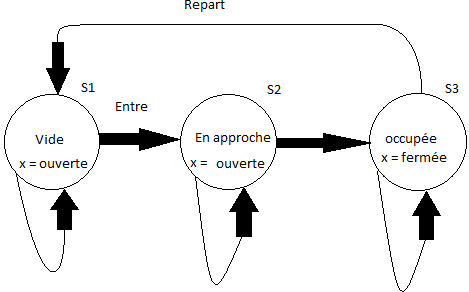
\includegraphics[scale=0.5]{graphe.png}
	\centering
	\caption{Modèle Kripke}
	\label{label-image3}
\end{figure}

\noindent Avec x étant une variable propositionnelle pour déterminer l'état des portes.\\
Un tel modèle est appelé \textit{Kripke Model}.\\
Par convention, le modèle \textit{Kripke} : $$K = (V, S, S_{0}, I, R)$$ \\
est le modèle \textit{Kripke} dont :
\begin{enumerate}
\item \textbf{V}\{ouverte, se ferme, fermée\} est un ensemble fini de propositions atomiques.
\item \textbf{S}\{vide, en approche, occupée\} est en ensemble fini d'état.
\item \textbf{$\textrm{S}_\textrm{0}$} est l'état initial.
\item \textbf{I : S $\rightarrow$ 2\up{V}} est la fonction qui lie chaque états avec les propositions qui y sont liées.
\item \textbf{R} est l'ensemble des relations entre chacun des états.
\end{enumerate}

\noindent Nous avons donc ici un graphe infini puisque celui-ci est cyclique. lorsqu'on transformera ce graphe en un arbre de recherche, nous aurons donc également un arbre infini. Faisons le travail de transformer ce graphe en un arbre : 
\begin{figure}[!h]
	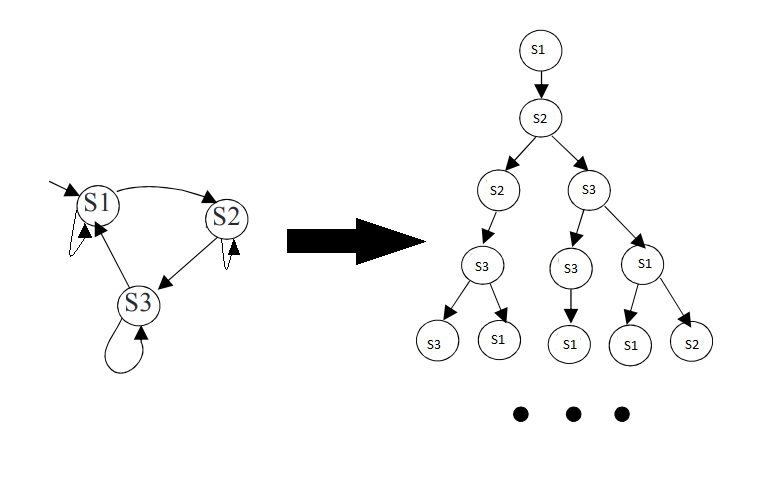
\includegraphics[scale=0.4]{kripke.png}
	\centering
	\caption{du Modèle Kripke à l'arbre de recherche}
	\label{label-image4}
\end{figure}

\noindent C'est maintenant grâce à de telles structures que nous allons pouvoir analyser notre système et vérifier que celui-ci soit infaillible.

\subsection{Computational Tree Logic (CTL)}

La syntaxe de la \textit{Computational Tree Logic} utilise des formule booléennes : \textit{True} et \textit{False} sont donc des formules \textit{CTL}.\\
Les variables propositionnelles sont des formules \textit{CTL}.\\
Ainsi, si $\varphi$ et $\psi$ sont des formules \textit{CTL} alors : $\lnot \varphi$, $\varphi \land \psi$ et $\varphi \lor \psi$ le sont aussi.\\

\noindent En plus de cela, plusieurs opérations sont également des formules \textit{CTL} : 

\begin{itemize}
\item EX $\varphi$ : $\varphi$ apparait dans un des états suivants.
\item EF $\varphi$ : Dans au moins un chemin, $\varphi$ apparait dans un état future.
\item EG $\varphi$ : Dans au moins un chemin, $\varphi$ apparait dans tous les états futures.
\item E[$\varphi \cup \psi$] : Dans au moins un chemin, $\varphi$ apparait jusqu'à ce que $\psi$ apparaisse. \\
\end{itemize}


\noindent Les opérations ici citées sont à chaque fois des "\textit{There exists}" (EX = Exists next), mais il existe également les opérations "\textit{ForAll}". \\
Ainsi, AX $\varphi$ : $\varphi$ apparait dans \textbf{tous} les états suivants.
AF, AG, A$\cup$ sont donc aussi des opérations valables.\\

\noindent Voici à titre d'exemple un schéma pour se donner une idée de ce que \textit{EF} et \textit{AF} signifient : 

\begin{figure}[!h]
	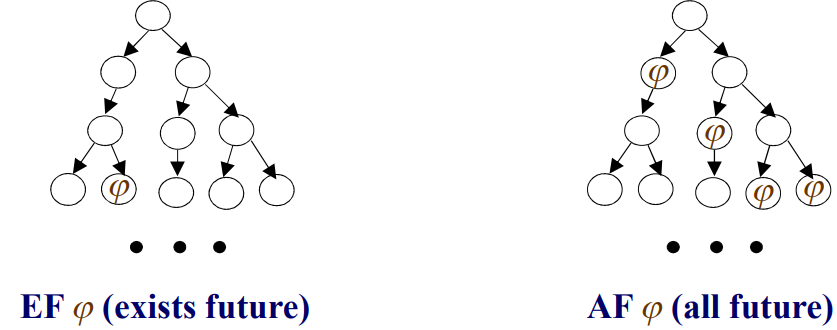
\includegraphics[scale=0.4]{F.png}
	\centering
	\caption{Exemple}
	\label{label-image5}
\end{figure}

\noindent A titre d'exemple toujours, essayons d'appliquer ces formules avec l'exemple de la figure \ref{label-image3}. \\
Propriétés validées : 
\begin{itemize}
\item (AX ouverte)($S_{1}$) : En effet, lorsqu'on démarre de $S_{1}$, on peut aller vers $S_{1}$ soit $S_{2}$, et la variable propositionnelle pour ces deux états est "ouverte".
\item (EF ouverte)($S_{3}$)
\item (AF fermée)($S_{1}$)\\
\end{itemize}

\noindent Propriétés non validées : 
\begin{itemize}
\item (AX fermée)($S_{3}$)\\
\end{itemize}


\noindent De ces opérateurs découlent pas mal de propriétés. En voici une liste non exhaustive : 
\begin{itemize}
\item $\lnot$ AX $\varphi \Leftrightarrow $ EX $\lnot \varphi$
\item $\lnot$ AF $\varphi \Leftrightarrow $ EG $\lnot \varphi$
\item AF $\varphi \Leftrightarrow $ A[true $\cup \ \varphi$]
\item AG $\varphi \Leftrightarrow \varphi \ \land$ AX AG $\varphi$
\item AF $\varphi \Leftrightarrow \varphi \ \lor$ AX AF $\varphi$
\item A[false $\cup \ \varphi$] $ \Leftrightarrow $ E[false $\cup \ \varphi$] = $\varphi$
\item A[$\varphi \ \cup \ \psi$] $ \Leftrightarrow \psi \ \lor$ ($\varphi \ \land$ AX A[$\varphi \ \cup \ \psi$])
\item E[$\varphi \ \cup \ \psi$] $ \Leftrightarrow \psi \ \lor$ ($\varphi \ \land$ EX E[$\varphi \ \cup \ \psi$])
\item A[$\varphi$ W $\psi$] $ \Leftrightarrow \lnot$ E[$\lnot \psi \ \cup$ ($\lnot \varphi \ \land \ \lnot \psi$)]\\
\end{itemize}

\noindent Maintenant que nous avons fait un tour non exhaustif de ce qu'était la syntaxe de \textit{CTL}, abordons la sémantique :  \\

\begin{itemize}
\item Soit $\varphi$ une formule \textit{CTL}, alors : $$K, s \vDash \varphi$$ signifie que $\varphi$ est vérifié à l'état \textbf{s}. La plupart du temps, K est omis puisque nous toujours au sein du même modèle \textit{Kripke}.\\
\item $\pi$ = $\pi\up{0} \pi\up{1} ...$ est un chemin.
\item $\pi\up{0}$ est l'état initial (la racine).
\item $\pi\up{i+1}$ est un des états succédant $\pi\up{i}$.\\
\end{itemize}

\noindent A nouveau, une série de propriétés découle des définitions précédentes : 
\begin{itemize}
\item AX $\varphi \Leftrightarrow \forall \pi \cdot \pi\up{1} \vDash \varphi$
\item EX $\varphi \Leftrightarrow \exists \pi \cdot \pi\up{1} \vDash \varphi$
\item AG $\varphi \Leftrightarrow \forall \pi \cdot \forall i \cdot \pi\up{i} \vDash \varphi$
\item EG $\varphi \Leftrightarrow \exists \pi \cdot \forall i \cdot \pi\up{i} \vDash \varphi$
\item AF $\varphi \Leftrightarrow \forall \pi \cdot \exists i \cdot \pi\up{i} \vDash \varphi$
\item EF $\varphi \Leftrightarrow \exists \pi \cdot \exists i \cdot \pi\up{i} \vDash \varphi$
\item A[$\varphi \ \cup \ \psi$]  $\Leftrightarrow \forall \pi \cdot \exists i \cdot \pi\up{i} \vDash 	\psi \land \forall j \cdot 0 \leq j < i \Rightarrow \pi\up{j} \vDash \varphi$
\item E[$\varphi \ \cup \ \psi$]  $\Leftrightarrow \exists \pi \cdot \exists i \cdot \pi\up{i} \vDash 	\psi \land \forall j \cdot 0 \leq j < i \Rightarrow \pi\up{j} \vDash \varphi$ \\
\end{itemize}

\noindent \underline{Définition} : Une formule \textit{CTL} est \textit{ACTL} si elle n'utilise que les connecteurs universels temporels (AX, AF, AG, AU).\\
\underline{Définition} : Une formule \textit{CTL} est \textit{ECTL} si elle n'utilise que les connecteurs existentiels temporels (EX, EF, EG, EU).\\
\underline{Définition} : Les formules \textit{CTL} qui ne sont ni \textit{ACTL} ni \textit{ECTL} sont appelées mixtes.\\

\noindent Grâce à la syntaxe et à la sémantique que nous avons évoqué, il est maintenant possible de parler de la sécurité et la vivacité d'un système.\\

\noindent \underline{Définition} : Un système sûre implique qu'il ne se passera jamais quelque chose de mauvais. AG $\lnot$ \textit{bad} \\
\underline{Définition} : Un système vivace implique que quelque chose de bien arrivera toujours. AG AF \textit{good}



\subsection{CTL Model Checking}


\end{document}